\documentclass[a4paper,twoside]{article}
\usepackage{blindtext}  
\usepackage{geometry}

% Chinese support
\usepackage[UTF8, scheme = plain]{ctex}

% Page margin layout
\geometry{left=2.3cm,right=2cm,top=2.5cm,bottom=2.0cm}


\usepackage{listings}
\usepackage{xcolor}
\usepackage{geometry}
\usepackage{amsmath}
\usepackage{float}
\usepackage{hyperref}

\usepackage{graphics}
\usepackage{graphicx}
\usepackage{subfigure}
\usepackage{epsfig}
\usepackage{float}

\usepackage{algorithm}
\usepackage[noend]{algpseudocode}

\usepackage{booktabs}
\usepackage{threeparttable}
\usepackage{longtable}
\usepackage{listings}
\usepackage{tikz}

% cite package, to clean up citations in the main text. Do not remove.
\usepackage{cite}

\usepackage{color,xcolor}

%% The amssymb package provides various useful mathematical symbols
\usepackage{amssymb}
%% The amsthm package provides extended theorem environments
\usepackage{amsthm}
\usepackage{amsfonts}
\usepackage{enumerate}
\usepackage{enumitem}
\usepackage{listings}

\usepackage{indentfirst}
\setlength{\parindent}{2em} % Make two letter space in the first paragraph
\usepackage{setspace}
\linespread{1.5} % Line spacing setting
\usepackage{siunitx}
\setlength{\parskip}{0.5em} % Paragraph spacing setting

% \usepackage[contents =22920202204622, scale = 10, color = black, angle = 50, opacity = .10]{background}

\renewcommand{\figurename}{图}
\renewcommand{\lstlistingname}{代码} 
\renewcommand{\tablename}{表格}
\renewcommand{\contentsname}{目录}
\floatname{algorithm}{算法}

\graphicspath{ {images/} }

%%%%%%%%%%%%%
\newcommand{\StudentNumber}{22920202204622}  % Fill your student number here
\newcommand{\StudentName}{熊恪峥}  % Replace your name here
\newcommand{\PaperTitle}{作业(三)}  % Change your paper title here
\newcommand{\PaperType}{算法设计与分析} % Replace the type of your report here
\newcommand{\Date}{2022年3月7日}
\newcommand{\College}{信息学院}
\newcommand{\CourseName}{算法设计与分析}
%%%%%%%%%%%%%

%% Page header and footer setting
\usepackage{fancyhdr}
\usepackage{lastpage}
\pagestyle{fancy}
\fancyhf{}
% This requires the document to be twoside
\fancyhead[LO]{\texttt{\StudentName }}
\fancyhead[LE]{\texttt{\StudentNumber}}
\fancyhead[C]{\texttt{\PaperTitle }}
\fancyhead[R]{\texttt{第{\thepage}页,共\pageref*{LastPage}页}}


\title{\PaperTitle}
\author{\StudentName}
\date{\Date}

\lstset{
	basicstyle          =   \sffamily,          % 基本代码风格
	keywordstyle        =   \bfseries,          % 关键字风格
	commentstyle        =   \rmfamily\itshape,  % 注释的风格,斜体
	stringstyle         =   \ttfamily,  % 字符串风格
	flexiblecolumns,                % 别问为什么,加上这个
	numbers             =   left,   % 行号的位置在左边
	showspaces          =   false,  % 是否显示空格,显示了有点乱,所以不现实了
	numberstyle         =   \zihao{-5}\ttfamily,    % 行号的样式,小五号,tt等宽字体
	showstringspaces    =   false,
	captionpos          =   t,      % 这段代码的名字所呈现的位置,t指的是top上面
	frame               =   lrtb,   % 显示边框
}

\lstdefinestyle{PythonStyle}{
	language        =   Python, % 语言选Python
	basicstyle      =   \zihao{-5}\ttfamily,
	numberstyle     =   \zihao{-5}\ttfamily,
	keywordstyle    =   \color{blue},
	keywordstyle    =   [2] \color{teal},
	stringstyle     =   \color{magenta},
	commentstyle    =   \color{red}\ttfamily,
	breaklines      =   true,   % 自动换行,建议不要写太长的行
	columns         =   fixed,  % 如果不加这一句,字间距就不固定,很丑,必须加
	basewidth       =   0.5em,
}

\algnewcommand\algorithmicinput{\textbf{Input:}}
\algnewcommand\algorithmicoutput{\textbf{Output:}}
\algnewcommand\Input{\item[\algorithmicinput]}%
\algnewcommand\Output{\item[\algorithmicoutput]}%

\begin{document}
	
%%%%%%%%%%%%%%%%%%%%%%%%%%%%%%%%%%%%%%%%%%%%
\makeatletter % change default title style
\renewcommand*\maketitle{%
	\begin{center} 
		\bfseries  % title 
		{\LARGE \@title \par}  % LARGE typesetting
		\vskip 1em  %  margin 1em
		{\global\let\author\@empty}  % no author information
		{\global\let\date\@empty}  % no date
		\thispagestyle{empty}   %  empty page style
	\end{center}%
	\setcounter{footnote}{0}%
}
\makeatother
%%%%%%%%%%%%%%%%%%%%%%%%%%%%%%%%%%%%%%%%%%%%
	
	
\thispagestyle{empty}

\vspace*{1cm}

\begin{figure}[h]
	\centering
	
\includegraphics[width=4.0cm]{logo.png}
\end{figure}

\vspace*{1cm}

\begin{center}
	\Huge{\textbf{\PaperType}}
	
	\Large{\PaperTitle}
\end{center}

\vspace*{1cm}

\begin{table}[h]
	\centering	
	\begin{Large}
		\renewcommand{\arraystretch}{1.5}
		\begin{tabular}{p{3cm} p{5cm}<{\centering}}
			姓\qquad 名 & \StudentName  \\
			\hline
			学\qquad号 & \StudentNumber \\
			\hline
			日\qquad期 & \Date  \\
			\hline
			学\qquad院 & \College  \\
			\hline
			课程名称 & \CourseName  \\
			\hline
		\end{tabular}
	\end{Large}
\end{table}

\newpage

\title{
	\Large{\textcolor{black}{\PaperTitle}}
}
	
	
\maketitle
	
\tableofcontents
 
\newpage
\begin{spacing}{1.2}

\section{题4.2}
算法\ref{algo:bmvoting}使用多数投票算法查找出现次数最多的元素。
\begin{algorithm}
	\caption{查找数组中出现次数最多的元素}
	\label{algo:bmvoting}
	\begin{algorithmic}[1]
		\Output{元组$(m,c)$,其中$m$是出现最多的元素,$c$是出现次数}
		\Procedure{FindMost}{$A$}     
		\State $c \gets 0$
		\State $m \gets 0$
		\For{$j \gets 1$ to $n$}
		\If{$c==0$}
		\State $c \gets 1$
		\State $m \gets A[j]$
		\EndIf
		\If{$A[j]==m$}
		\State $c \gets $c+1
		\Else
		\State $c \gets $c-1
		\EndIf
		\EndFor
		
		\State $c \gets 0$
		\For{$j \gets 1$ to $n$}
		\If{$A[j]==m$}
		\State $c \gets $c+1
		\EndIf
		\EndFor
		\Return (m,c)
		\EndProcedure
		
	\end{algorithmic}
\end{algorithm}	

该算法前10行使用投票法找到出现次数最多的元素,然后统计出现的次数。时间复杂度是$O(n)$,空间复杂度是$O(1)$。


\section{题4.4}

$Perm(m)$的循环不变式是

$$
L_m=\mbox{每次执行$Perm(m)$前,$P[1\dots m-1]$是$m-1$个元素的一个排列。}
$$

\textbf{初始:}当$m=1$时,$P[1\dots 0]$中是0个元素的排列,即空集。

\textbf{归纳:}调用$Perm(m)$时,$P[1\dots m-1]$是$m-1$个元素的一个排列,算法$Perm(m)$将$P[j]$中放入第$m+1\dots n$中的一个元素,得到$m$个数字的排列。

\textbf{终止:}当$m=n$时,即$m=n+1$执行前,$P[1\dots n]$是$n$个元素的一个排列。

\section{题4.6}

\textbf{初始:}$GeneratingPerm2$第一次调用$Perm2(n)$时,$P[1\dots n]$有$n$个$0$。

\textbf{归纳:}若调用$Perm2(m)$时有$m$个$0$,$Perm2(m)$先在其中一个$0$的位置以$m$替代$0$,然后调用$Perm2(m-1)$,此时有$m-1$个$0$。

因此在每一次调用$Perm2(m)$时$P$中都有$m$个$0$。

$Perm(2)$中的$for$循环将每一个$0$的位置以$m$替代$0$然后调用$Perm2(m-1)$,因此$Perm2(m-1)$调用了$m$次。

\section{题4.11}

令

$$
n=2^m
$$

则

$$
S(m)=T(2^m)=2T(2^{\frac{m}{2}})+1=2S(\frac{m}{2})+1
$$

猜测$S(m)=O(m)$,则需要证$S(m)\le cn-b$

\textbf{当$m=1$},$S(m)=1\le c-b$,当$c \ge 1+b$。

\textbf{若$S(\frac{m}{2})\le c\frac{m}{2}-b$},则

\begin{align*}
	S(m)&=2S(\frac{m}{2})+1 \\
	&=2c \frac{m}{2}+1-2b \\
	& \le cm-b
\end{align*}

当

$$
b \ge 1
$$

所以

$$
S(m) \le cm \iff S(m)=O(m)
$$

则

$$
T(n)=T(2^m)=S(m)=O(m)=O(\log n)
$$

\section{题4.12}

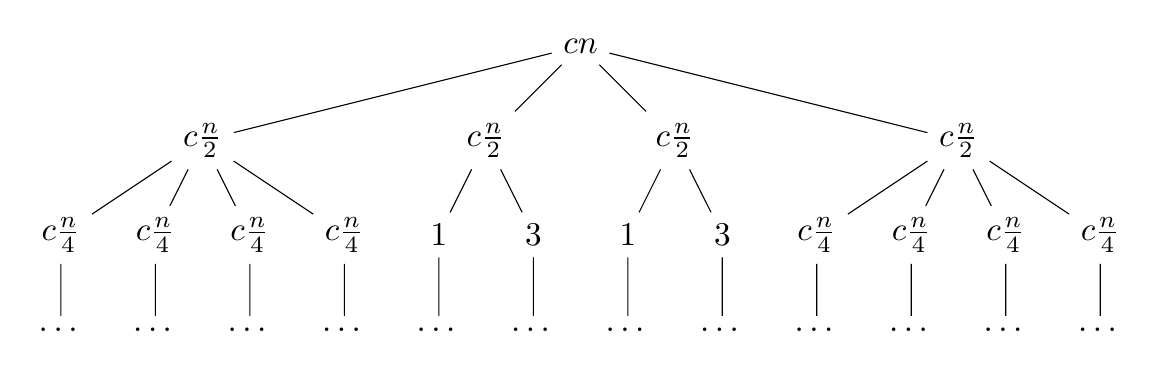
\begin{tikzpicture}
	[thin,scale=0.8, every node/.style={scale=1.2}]
	\node {$cn$}
	child {node {$c\frac{n}{2}$}
		child {node {$c\frac{n}{4}$}
			child {node {$\dots$}}
		}
		child {node {$c\frac{n}{4}$}
			child {node {$\dots$}}
		}
		child {node {$c\frac{n}{4}$}
			child {node {$\dots$}}
		}
		child {node {$c\frac{n}{4}$}
			child {node {$\dots$}}
		}
	}	
	child [missing] {}	
	child [missing] {}	
	child { node {$c\frac{n}{2}$}
		child {node {1}
			child {node {$\dots$}}
		}
		child {node {3}
			child {node {$\dots$}}
		}
	}	
	child [missing] {}	
	child { node {$c\frac{n}{2}$}
	child {node {1}
			child {node {$\dots$}}
		}
		child {node {3}
			child {node {$\dots$}}
		}
	}
	child [missing] {}	
	child [missing] {}	
	child { node {$c\frac{n}{2}$}
		child {node {$c\frac{n}{4}$}
			child {node {$\dots$}}
		}
		child {node {$c\frac{n}{4}$}
			child {node {$\dots$}}
		}
		child {node {$c\frac{n}{4}$}
			child {node {$\dots$}}
		}
		child {node {$c\frac{n}{4}$}
			child {node {$\dots$}}
		}
	};
\end{tikzpicture}


由树状图可得$k=\log_2 n$

则

\begin{align*}
	& cn + 4 \cdot \frac{1}{2} n + 16 \cdot \frac{1}{16} n + \dots \\
	&= n \sum_{i=1}^{\log_2 n} 2^i \\
	&= n \frac{2(1-n)}{1-2} \\
	&= 2n^2-2n
\end{align*}

因此

$$
T(n)=O(n^2)
$$

\textbf{证明: $T(n) \le kn^2-bn$}

\textbf{当}$n=1$,$T(n)=c \le k-b$,当$k \ge c+b$

\textbf{若}$T(\frac{n}{2})<k{(\frac{n}{2})}^2-b\frac{n}{2}$

\begin{align*}
T(n) & \le 4 k{(\frac{n}{2})}^2 -b\frac{n}{2} + cn \\
 &= kn^2 - (\frac{b}{2}-c)n \\
 & \le kn^2 - bn
\end{align*}

当

$$
b \le 2c
$$

\section{Leetcode 144}

\subsection{思路分析}

求先序遍历,就先输出根节点的值,然后对左右子树分别进行先序遍历。运行结果如图\ref{fig:lc144}。代码如\ref{code:lc144},递归的终止条件是左右子树都是空。具体实现见\nameref{sec:code}。

\subsection{运行结果}

\begin{figure}[h]
	\centering
	\label{fig:lc144}
	\caption{运行结果}
	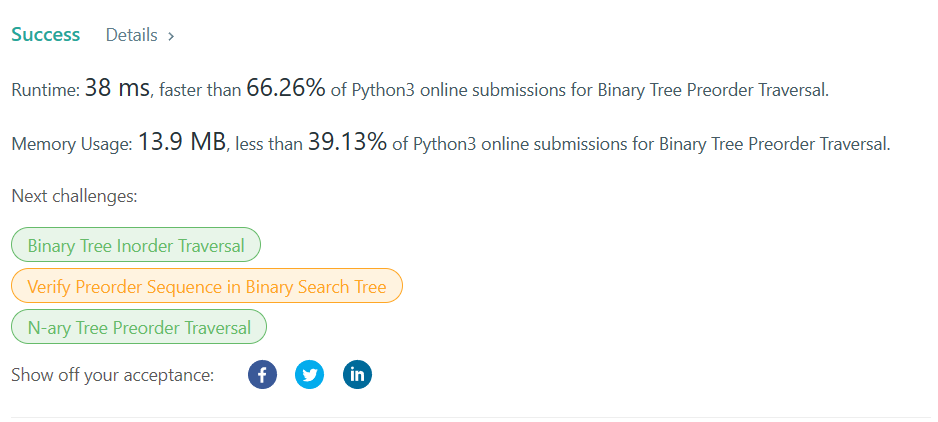
\includegraphics[width=0.8\linewidth]{lc144.png}
\end{figure}

\section{Leetcode 236}

LCA是一种有各种算法的问题。常见的方法比如使用了并查集的Tarjan算法能较快地给出多组LCA查询的答案。但我写了一个暴力的算法,因为我想体验一下暴力算法的写法。

\subsection{思路分析}

首先假设有如图\ref{fig:btree}(a)所示的二叉树,假设我们对点$h$和$d$求LCA,那么我们先对节点递归地标注高度,并求出节点的父节点,然后得到\ref{fig:btree}(b),之后按照如下方法进行迭代

\begin{itemize}
	\item 先让高度较低(高度值较大的节点沿父节点方向向上移动到两个节点处在同一层
	\item 两节点同时向上移动直到首次达到相等
\end{itemize}

然后就得到了LCA是$a$的答案。按照这个思路实现代码\ref{code:lc236},具体见\nameref{sec:code}。

\subsection{运行结果}

运行结果如图\ref{fig:lc236}。可以发现暴力算法确实运行较慢,而且并不比Tarjan算法好写,看来还是写Tarjan算法比较好。
\begin{figure}
	\centering
	\caption{一棵二叉树}
	\label{fig:btree}
	\subfigure[原始二叉树]{
	\begin{minipage}[t]{0.4\linewidth}
		\centering
		\begin{tikzpicture}
			[thick,scale=0.8, every node/.style={scale=1}]
			\node {a}
			child {node {b}
				child {node {c}}
				child {node {d}}
			}	
			child [missing] {}	
			child {node {e}
				child {node {f}}
				child { node {g}
					child {node {h}}
					child {node {i}
						child {node {j}}
					}
				}	
			};
		\end{tikzpicture}
	\end{minipage}}
	\subfigure[预处理后的二叉树]{
	\begin{minipage}[t]{0.4\linewidth}
		\centering
		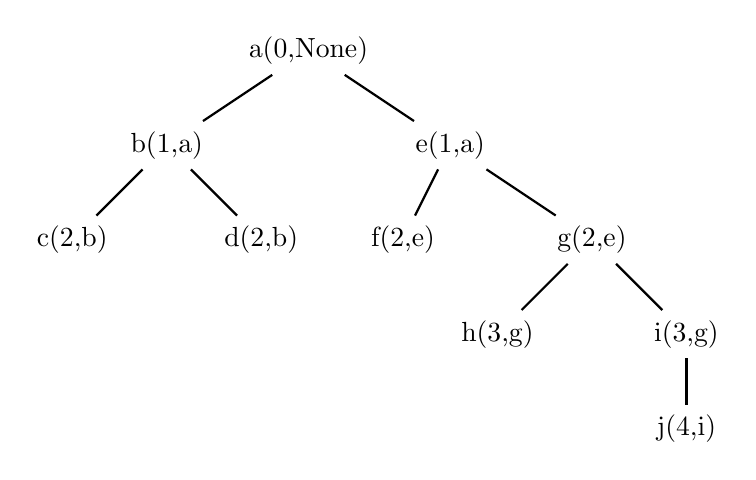
\begin{tikzpicture}
			[thick,scale=0.8, every node/.style={scale=1}]
			\node {a(0,None)}
			child {node {b(1,a)}
				child [missing] {}	
				child {node {c(2,b)}}
				child [missing] {}	
				child {node {d(2,b)}}
				child [missing] {}	
			}	
			child [missing] {}	
			child [missing] {}	
			child {node {e(1,a)}
				child [missing] {}	
				child {node {f(2,e)}}
				child [missing] {}	
				child { node {g(2,e)}
					child {node {h(3,g)}}
					child [missing] {}	
					child {node {i(3,g)}
						child {node {j(4,i)}}
					}
				}	
			};
		\end{tikzpicture}
	\end{minipage}}
	
\end{figure}

\begin{figure}[htbp]
	\centering
	\label{fig:lc236}
	\caption{运行结果}
	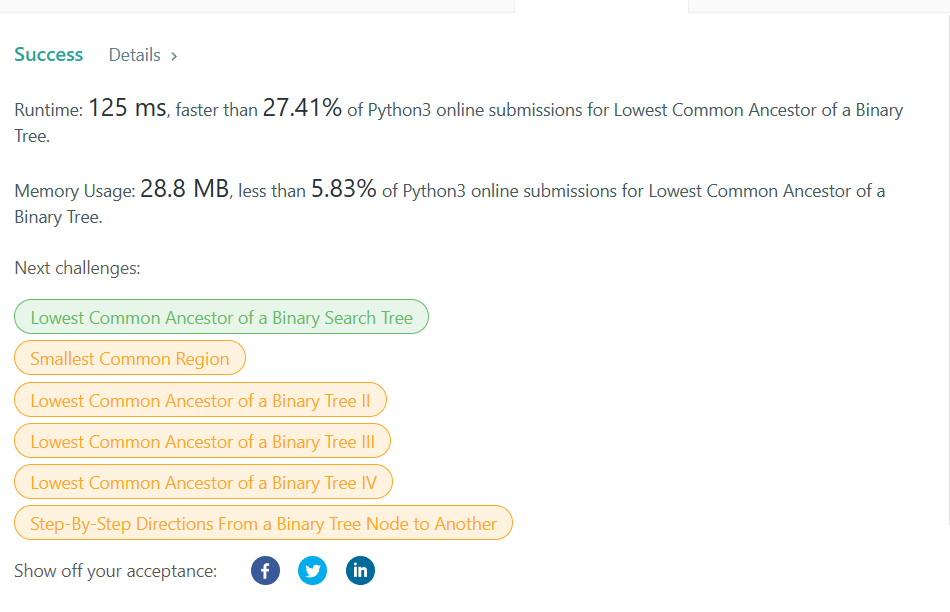
\includegraphics[width=0.8\linewidth]{lc236.png}
\end{figure}


\newpage
\clearpage

\appendix


\section{附录:编程题代码}
\label{sec:code}

\begin{lstlisting}[language=Python,numbers=left,style=PythonStyle,caption=求先序遍历,label={code:lc144}]
class Solution:
	def __init__(self):
		self.list = []
	
	def traversal(self, root: Optional[TreeNode]):
		if root is None:
			return
		
		self.list.append(root.val)
		self.traversal(root.left)
		self.traversal(root.right)
	
	def preorderTraversal(self, root: Optional[TreeNode]) -> List[int]:
		self.traversal(root)
		return self.list
	
\end{lstlisting}

\begin{lstlisting}[language=Python,numbers=left,style=PythonStyle,caption=求LCA,label={code:lc236}]
class Solution:
	def __init__(self):
		self.heights = dict()
	
	def height(self, root: 'TreeNode', anc: Optional[TreeNode], h):
		root.ancestor = anc
		self.heights[root] = h
	
	if root.left is not None:
		self.height(root.left, root, h + 1)
	
	if root.right is not None:
		self.height(root.right, root, h + 1)

	def lowestCommonAncestor(self, root: 'TreeNode', p: 'TreeNode', q: 'TreeNode') -> 'TreeNode':
		self.height(root, None, 1)
		
		if self.heights[p] == self.heights[q]:
			while p.val != q.val:
			p = p.ancestor
			q = q.ancestor
		
		return p
		
		(low, high, high_h) = (p, q, self.heights[q]) if self.heights[p] > self.heights[q] else (q, p, self.heights[p])
		
		while self.heights[low] > high_h:
			low = low.ancestor
		
		while not (low is None) and not (high is None) and low.val != high.val:
			low = low.ancestor
			high = high.ancestor
		
		return low
\end{lstlisting}


\end{spacing}
\end{document}